\chapter{Methodology}\label{cha:method}

The goals of this research requires the development of several components, chiefly among them a pollen dataset and object detection model.
Section~\ref{sec:method-dataset} covers the data collection and Section~\ref{sec:method-arch} details the model architecture.
As a prerequisite for being able to analyze sharpness, an objective sharpness measure is needed.
A theoretical background for this is given in Section~\ref{sec:method-sharpness}.
Finally, the experimental setup as well as the experiments themselves are explained in Sections~\ref{sec:method-exp-setup} \&~\ref{sec:method-experiments}, respectively.

\section{Data}\label{sec:method-dataset}

\begin{figure}[htbp]
  \centering
  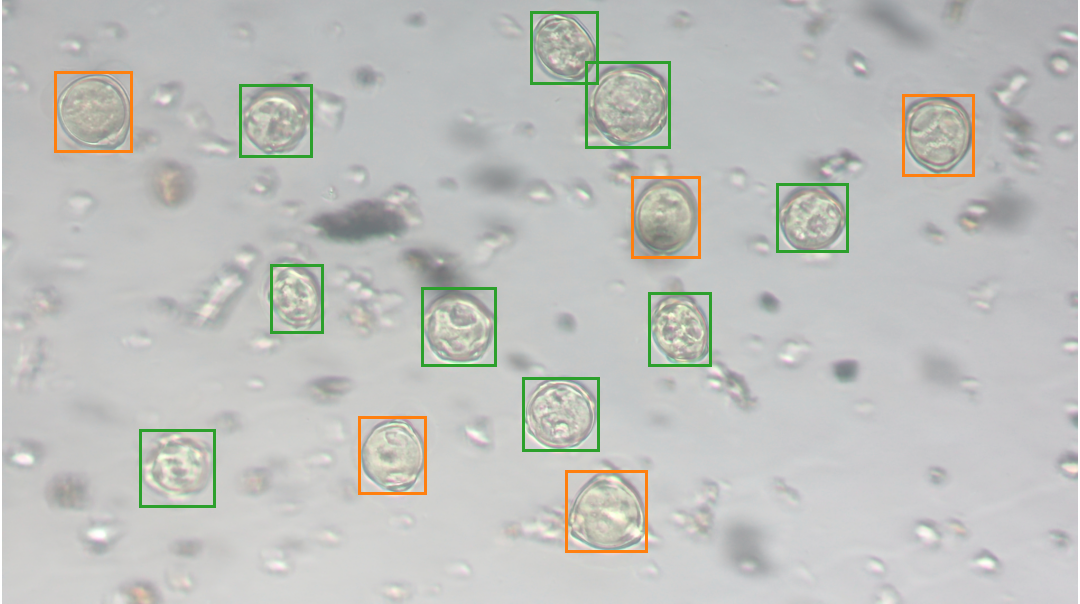
\includegraphics[width=0.8\textwidth]{figs/method/Snap-057.png}
  \caption[Dataset example]{Example from the dataset with ground truth bounding boxes drawn.
The image contains two classes: \textcolor{corylus}{corylus}, and \textcolor{alnus}{alnus}.}\label{fig:dataset-sample}
\end{figure}

The results presented in Chapter~\ref{cha:results} are trained on data sourced from the Norwegian Asthma and Allergy Association, who have, since 1980, tracked the amount of air born pollen in Norway.
Pollen is collected with traps where air is continually sucked though a small slit and is redirected over an adhesive strip.
The strip is moved across the slit, exposing different sections throughout the day.
Pollen grains and other air born particulates adhere to the strip, which is then analyzed under a microscope.
Only pollen grains from a subset of species are actively tracked.

Three microscope slides have been imaged using a digital optical microscope producing a set of 701 raster images with a size of \(1080\by 1920\) pixels and three channels; red, green, and blue.
The resolution of each image is \(\SI{0.183}{\micro\metre\per\pixel}\).
Each image has been labeled in collaboration with the experts to produce a valid and correct ground truths.
In total, three different species have been classified, namely \textit{poaceae}, \textit{corylus}, and \textit{alnus}, known in English as Grasses, Hazel, and Alder, respectively.
A labeled example is given in Figure~\ref{fig:dataset-sample}.
A summary of the dataset is given in Table~\ref{tab:dataset}.

\begin{table}[htbp]
  \caption[Class distribution across the dataset]{Distribution of class labels across the 701 sample images of the pollen dataset.}\label{tab:dataset}
  \centering
  \begin{tabular}{lrrr} \toprule
                      & Poaceae & Corylus & Alnus \\ \midrule
    Number of labels  & 5600    & 262     & 522 \\
    Proportion        & 87.7\%  & 4.1\%   & 8.2\% \\ \bottomrule
  \end{tabular}
\end{table}

Many of the images are taken from the same view point, but with the focus plane set to different grains.
The ground truth labels are drawn for all present pollen grains, regardless of the how blurred they appear.
This is done so that the dataset may be modified for the purpose of analyzing sharpness and model performance in regards to \textit{RQ2}.

As opposed to more general object detection tasks, where there is a large variance in both the apparent size and shape of objects within an image, this dataset is much more regular.
Looking at Figure~\ref{fig:aspect}, the grains are mostly circular in shape and between 100 and 150 pixels wide.

\begin{figure}[htb]
  \centering
  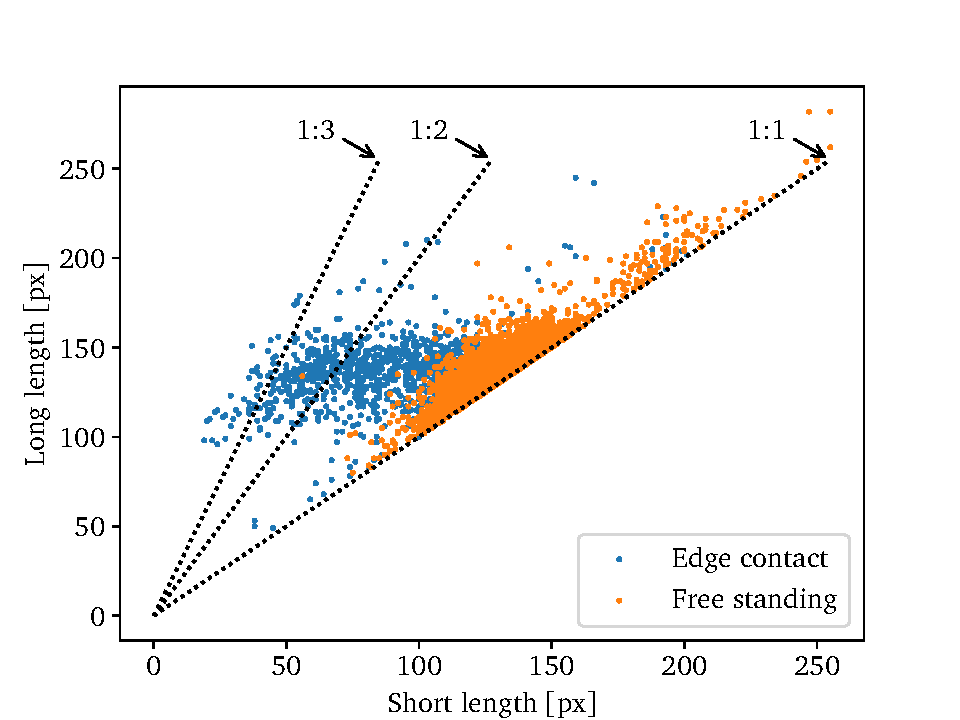
\includegraphics[width=0.9\textwidth]{figs/method/aspect_ratio.pdf}
  \caption[Aspect ratios in the dataset]{The widths and heights of all ground truth boxes are plotted, longest against shortest.
The lines denote the three aspect ratios used in the default boxes of the SSD model.
Grains marked `Edge contact' are those in direct contact with the edge of the image and are most likely partially cropped out of frame.
The grains are all quite regular in both shape and size}\label{fig:aspect}
\end{figure}

\section{Sharpness Measure}\label{sec:method-sharpness}
Analyzing how the sharpness of pollen grains affects detection performance requires an objective sharpness measure.
This section details the chosen method of measuring local sharpness of pollen grains within sample images.
The measure is based on Fourier analysis and its performance has been tested on the training data.

\subsection{Fourier analysis}
\done{Add axes to images\newline explain frequencies better}
Fourier analysis describes the general method of utilizing the Fourier transform to analyze the component frequencies present is some signal.
For the purpose of Fourier analysis, imagine the image as a collection of signals, each of which describe the change in brightness value when traveling across the image in some direction.
For an \(M\by N\) image, the two-dimensional Discrete Fourier Transform is defined as follows,

\begin{equation}
  F(u,v) = \sum_{m=0}^{M}\sum_{n=0}^{N}f(m,n)\,e^{-i2\pi\left(u\frac{m}{M}+v\frac{n}{N}\right)}
\end{equation}%
\begin{equation*}
  e^{-i2\pi\left(ux+vy\right)} = \cos 2\pi\left(ux+vy\right) + i\sin 2\pi\left(ux+vy\right) 
\end{equation*}
where \(f(m,n)\) is the spatial domain of the image, and the exponential term is the basis function at each point of \(F(u,v)\) in the Fourier domain.
Taking the Fourier transform of an image then produces a 2-dimensional matrix where the intensity of each element represents a the coefficient of a 2-dimensional sinusoid basis function of the image.
Figure~\ref{fig:fourier-sinusoid} visualizes what the basis functions can look like and demonstrates exactly what is encoded in the Fourier spectrum.

\begin{figure}[htbp]
  \centering
  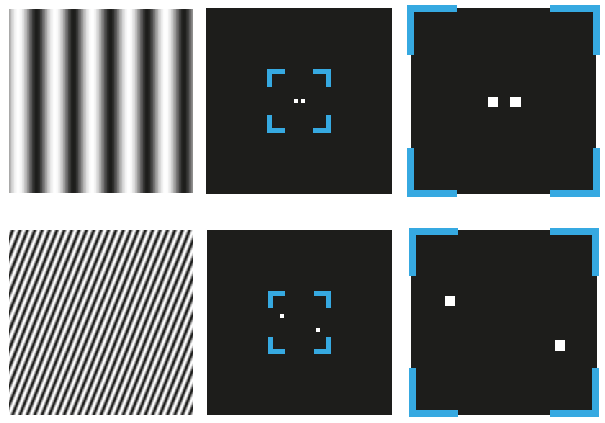
\includegraphics[width=0.8\textwidth]{figs/method/fourier/fourier-sinusoid.pdf}
  \caption[Fourier transform of sinusoid]{The figure shows two 2D sinusoid basis functions and their Fourier transform.
The active components in the transform have been enlarged so as to make them visible in print.
When unmodified, only a single pixel and its reflection about the origin is active.}\label{fig:fourier-sinusoid}
\end{figure}

Figure~\ref{fig:fourier-demo} shows the Fourier transform of various inputs.
The transforms are shifted, such that \(F(0,0)\) is in the center of the transform.
The maximum frequency that can be represented in the spacial domain is a 2 pixel wide stripe pattern going from minimum to maximum brightness.
\(u\) and \(v\) represent the number of oscillations in each direction of the basis function so the maximum frequency gives \(M/ 2\) and \(N/ 2\) oscillations, respectively.
The directionality of the Fourier transform is demonstrated in the first two examples.
Squares decompose into a set on sinusoids, all moving is the same two directions.
The coefficient of each component is encoded in the intensity of the pixel.
In all the examples the lower frequency components dominate, which lights up the center region.
The last two examples demonstrate how blurring an image eliminates the higher frequencies from the Fourier domain.

\begin{figure}[htbp]
  \centering
  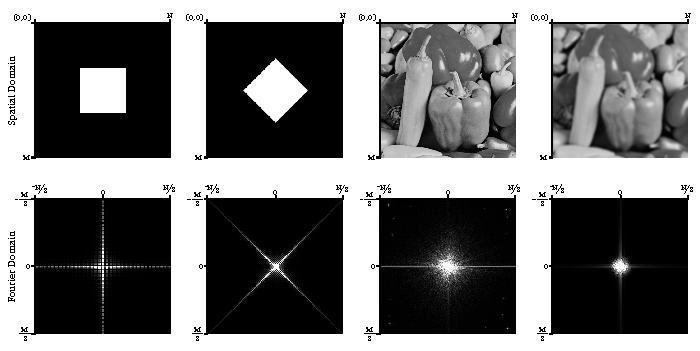
\includegraphics[width=\textwidth]{figs/method/fourier/fourier-examples.pdf}
  \caption[Demonstration of the Fourier transform]{
    Demonstration of the Fourier transform.
The bottom row shows the center-shifted discrete Fourier transform of the corresponding image in the top row.
The Fourier spectra mapped to grayscale values with a truncated linear amplitude mapping which is scaled to compensate for the otherwise dominating center component.}\label{fig:fourier-demo}
\end{figure}

Using the Fourier spectrum to measure sharpness follows from the realization that there is a strong relationship between the sharpness of an image in the spatial domain and the distribution of frequency components in the frequency domain.
Sharp features produce high frequencies while blur smooths out the changes in brightness, lowering the frequencies.
Figure~\ref{fig:fourier} shows three different pollen grains, captured with progressively more blur.
By visual inspection it is clear that as the perceived blur increases the amount of high frequency components also decreases.


\begin{figure}[htbp]
  \centering
  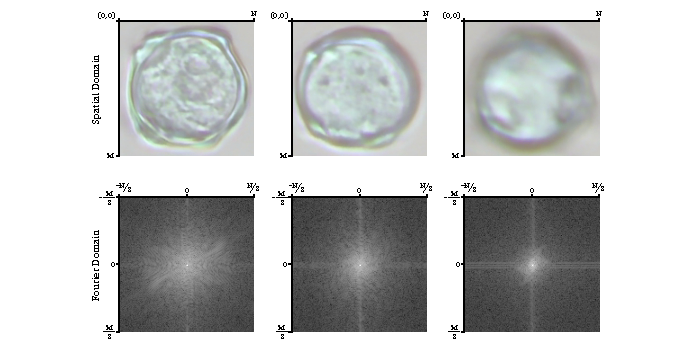
\includegraphics[width=\textwidth]{figs/method/fourier/fourier-pollen.pdf}
  \caption[Fourier spectrum]{Pollen grains and their corresponding centered Fourier spectrum.
The Fourier spectra are log scaled so that the higher frequencies become visible.}\label{fig:fourier}
\end{figure}

\subsection{Measuring sharpness}
The problem then is to decide how to encode this change in frequency distribution as a scalar sharpness measure.
\citeauthor{de2013image} propose a simple method which counts the number of components in the Fourier spectrum having a value above a certain threshold.
The operation is described in Equation (\ref{eq:sharp}).


\begin{equation}\label{eq:sharp}
  \begin{split}
    \mathbf{X} &= \mathcal{F}(a),\quad a\in \mathbb{Z}^{M\by N}\\
    T_H &= \sum_{x\in\mathbf{X}}[x\ge\mu],\quad \mu=\frac{\max \mathbf{X}}{1000}\\
    S &= \dfrac{T_H}{M\cdot N}
  \end{split}
\end{equation}

Here \(\mathcal{F}\) is the discrete the Fourier transform operating on an input image \(a\), which is a \(M\by N\) matrix of integers.
The phase component of the complex valued output is ignored, leaving \(\mathbf{X}\) to contain only the magnitude of the frequency components.
The scaling factor of the threshold value, \(\mu \), was found to produce good results on the data, without modification. \(S\) is the sharpness measure.

Validating the sharpness measure is an important task.
The weight of any argument made based on analysis using this measure is predicated on its soundness.
There are many different approaches to this, one of which is to compare the objective measure with subjective measurements of perceived sharpness on a subset of the training data.

\subsection{Evaluating the sharpness measure}
The basis of the evaluation is a new dataset created from a small random subset of the training examples.
Each ground truth is then given sharpness scores based on perceived sharpness and the objective measure.
Determining perceived sharpness of a pollen grain with high fidelity was found to be highly subjective and non-reproducible with repeated independent scoring, so a simple classification was instead performed.
Images where separated into three classes representing perceived sharpness.
Figure~\ref{fig:fourier} gives examples of the classes with the top left image being the sharpest (class 3) and the top right image being the blurriest (class 1).
A total of 316 pollen grains where evaluated, the distribution of their classes is given in Table~\ref{tab:sharpness}

\begin{table}[htbp]
  \caption[Sharpness dataset distribution]{Distribution of classes across the sharpness evaluation dataset.}\label{tab:sharpness}
  \centering
  \begin{tabular}{lrrr} \toprule
    & blurry [1] & partly [2] & sharp [3]  \\ \midrule
    Number of labels & 108 & 93  & 115 \\
    Share            & .34 & .30 & .36 \\ \bottomrule
  \end{tabular}
\end{table}

\begin{figure}[htbp]
  \centering
  \begin{subfigure}[t]{0.48\textwidth}
    \centering
    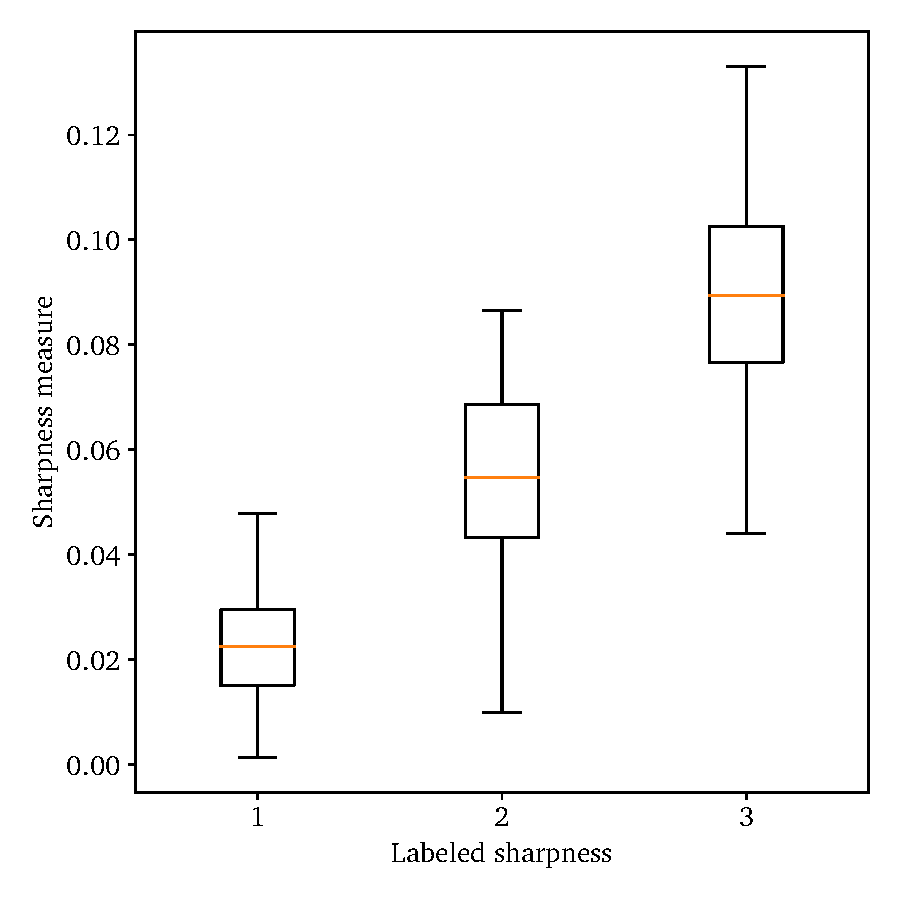
\includegraphics[width=\textwidth]{figs/method/box.pdf}
    \caption{Box plot}\label{fig:sharpness-box}
\end{subfigure}%
\hfill
\begin{subfigure}[t]{0.49\textwidth}
  \centering
  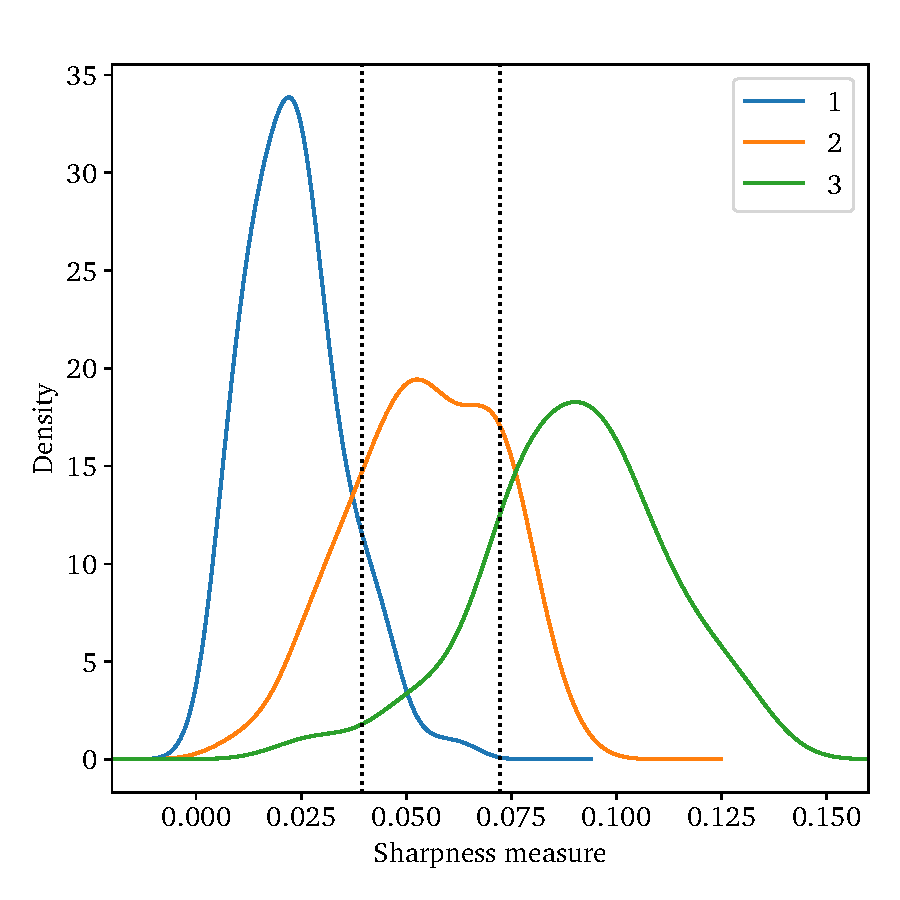
\includegraphics[width=\textwidth]{figs/method/qden.pdf}
  \caption{Density plot}\label{fig:sharpness-qden}
\end{subfigure}
  \caption[Sharpness measure separability]{The sharpness measure grouped by class label.
There is a large overlap between adjacent classes, but the IQRs in (a) are clearly separated.
The correlation between perceived and measured sharpness is also clear.}\label{fig:sharpness}
\end{figure}

Figure~\ref{fig:sharpness} shows a clear correlation between the mean of the distribution, and the perceived sharpness.
The overlap is to be expected, given the mapping from a continuous predictor onto a categorical label.
To further evaluate the performance of the sharpness measure a very simple decision tree model is constructed, and its ability to differentiate between the classes is tested.
The model achieved a test accuracy of 83.5\%.

Figure~\ref{fig:sharpness-all} shows the computed the sharpness of every ground truth in the dataset in a density plot, visualizing the approximate distribution.
As expected, most of the ground truths fall into the sharpest category, but there is a spread, allowing for the analysis of the relationship between sharpness and model performance.

\begin{figure}[htbp]
  \centering
  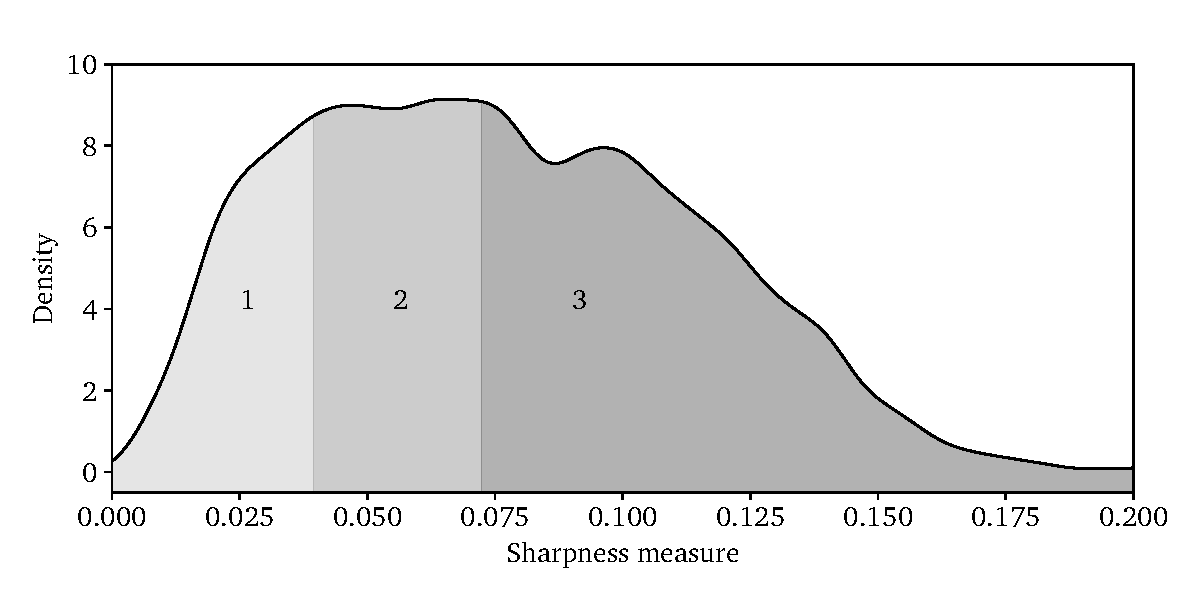
\includegraphics[width=0.9\textwidth]{figs/method/sharpness_all.pdf}
  \caption[Distribution of sharpness across entire dataset]{Density plot showing the sharpness of all pollen grains in the dataset \((N=6384)\).
The shaded sections indicate the distribution of sharpness classes, if the dataset is classified with the evaluation model.
As expected, most grains fall into the sharpest category.}\label{fig:sharpness-all}
\end{figure}

\section{Architecture}\label{sec:method-arch}

The model that has been implemented is the Single Shot Multibox Detector, a brief explanation of which was given in Section~\ref{sec:ssd}.
This section gives a more thorough explanation of the model and its implementation, with a focus on the changes that have been made from the original.
Most of these changes are motivated by more recent research featured in newer models.
The reasoning behind choosing a now relatively old model framework is mostly based on its architecture, which lends itself to alteration and simplification.


The implementation is based on an implementation by NVIDIA\footnote{Released under the Apache 2.0 License, \href{https://github.com/NVIDIA/DeepLearningExamples/tree/master/PyTorch/Detection/SSD}{URL:\\ } \url{https://github.com/NVIDIA/DeepLearningExamples/tree/master/PyTorch/Detection/SSD}}, the basic structure is shown in Figure~\ref{fig:model}.
The implementation can be divided into four parts.
A feature extraction network first transforms the input image into a set of high level feature maps, which are then fed into an \textit{auxiliary structure} which gradually steps down the dimensions of the feature map and in the process creates a set of source feature maps.
Two detection structures then consume the source feature maps which produces the final predictions.
One set of filters produces class confidence scores, and one produces bounding box regressions.

\subsection{Model}
The model comprises three distinct parts, a feature extraction network transferred from a pre-trained model, an auxiliary structure which creates a set of feature maps, and a detection structure which creates the bounding box regressions and class predictions.
The model is purely convolutional with no fully connected layers.

The feature extractor can be any classification network that can produce a feature map of the correct dimensions.
In the original paper the VGG-16 network is used\ \parencite{simonyan2015deep} without any particular justification as to why.
ResNet-34 is used in the baseline configuration.
The main reason for this is its superior performance over VGG, and the ease with which it integrates with the auxiliary structure\ \parencite{he2015deep}.
ResNet-34 is the largest of the ResNet family which fits on the GPU used for most of the experimentation.
PyTorch offers canonical implementations of the most popular pre-trained models as part of their API\@.

\begin{figure}[htb]
  \centering
  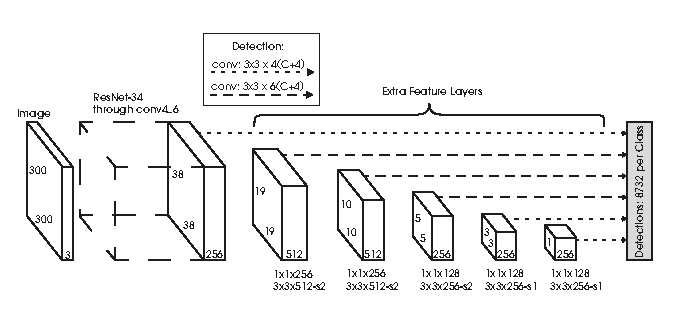
\includegraphics[width=0.9\textwidth]{figs/method/model.pdf}
  \caption[Model architecture overview]{Overview of the general structure of the model.
The figure is inspired by the one given in the original paper, but has been modified to reflect the alterations that have been made, and to highlight exactly how bounding box and class predictions are calculated with convolution.
The horizontal lines denote the detection structure comprised of \(3\by 3\) convolutions for class confidences and bounding box regressions.
Here \textsf{C} is the number of classes including one for background}\label{fig:model}
\end{figure}
\done{Show seperation of loc vs class parts in Figure}
The auxiliary structure is implemented as a sequence of blocks where the output of each block is a feature map which is consumed by the detection structure.
Each block contains two convolutional layers, as specified in Figure~\ref{fig:model}.
Batch normalization is used after each convolution and ReLU is used as the activation function.

The detection structure is implemented as a sequence of distinct layers, each of which runs over one of the intermediate feature maps from the auxiliary structure.
Each localizing layer has four filters per default box, one for each of the regression parameters.
Similarly, the class prediction layers have \(C\) filters per box, one for each class with an additional layer for the background.

When executing the forward pass through the model the input is first passed through the feature extractor, it is then passed through each block of the auxiliary structure, saving each feature map.
The final output is then generated by running each feature map through the corresponding localization and classification block.
All the outputs from the localization and classification layers are concatenated, producing two output tensors.
The dimensions are \(\left(B,4,D\right) \) and \(\left(B,C,D\right) \) for the localization and classification outputs, respectively.
Here \(B\) is the batch size and \(D\) is the number of default boxes.

\subsection{Default boxes}

The fundamental objective of the model is evaluating a predefined set of default boxes.
Each location of a feature map forms the basis for a small amount of default boxes of fixes size and aspect ratio.
In Figure~\ref{fig:defaults} the center element of the \(5\by 5\) feature map is responsible for evaluating the 4 drawn default boxes; 2 scaled squares in orange, and 2 boxes with a 1:2 aspect ratio, in blue.
The default boxes are scaled independently from the size of the elements of the feature map, but there is a correlation.
Because of the depth of the feature extraction network leading into the feature layers, the receptive field of all elements in every feature map is the entire input.%
\begin{wrapfigure}[14]{R}{0.4\textwidth}
  \centering
  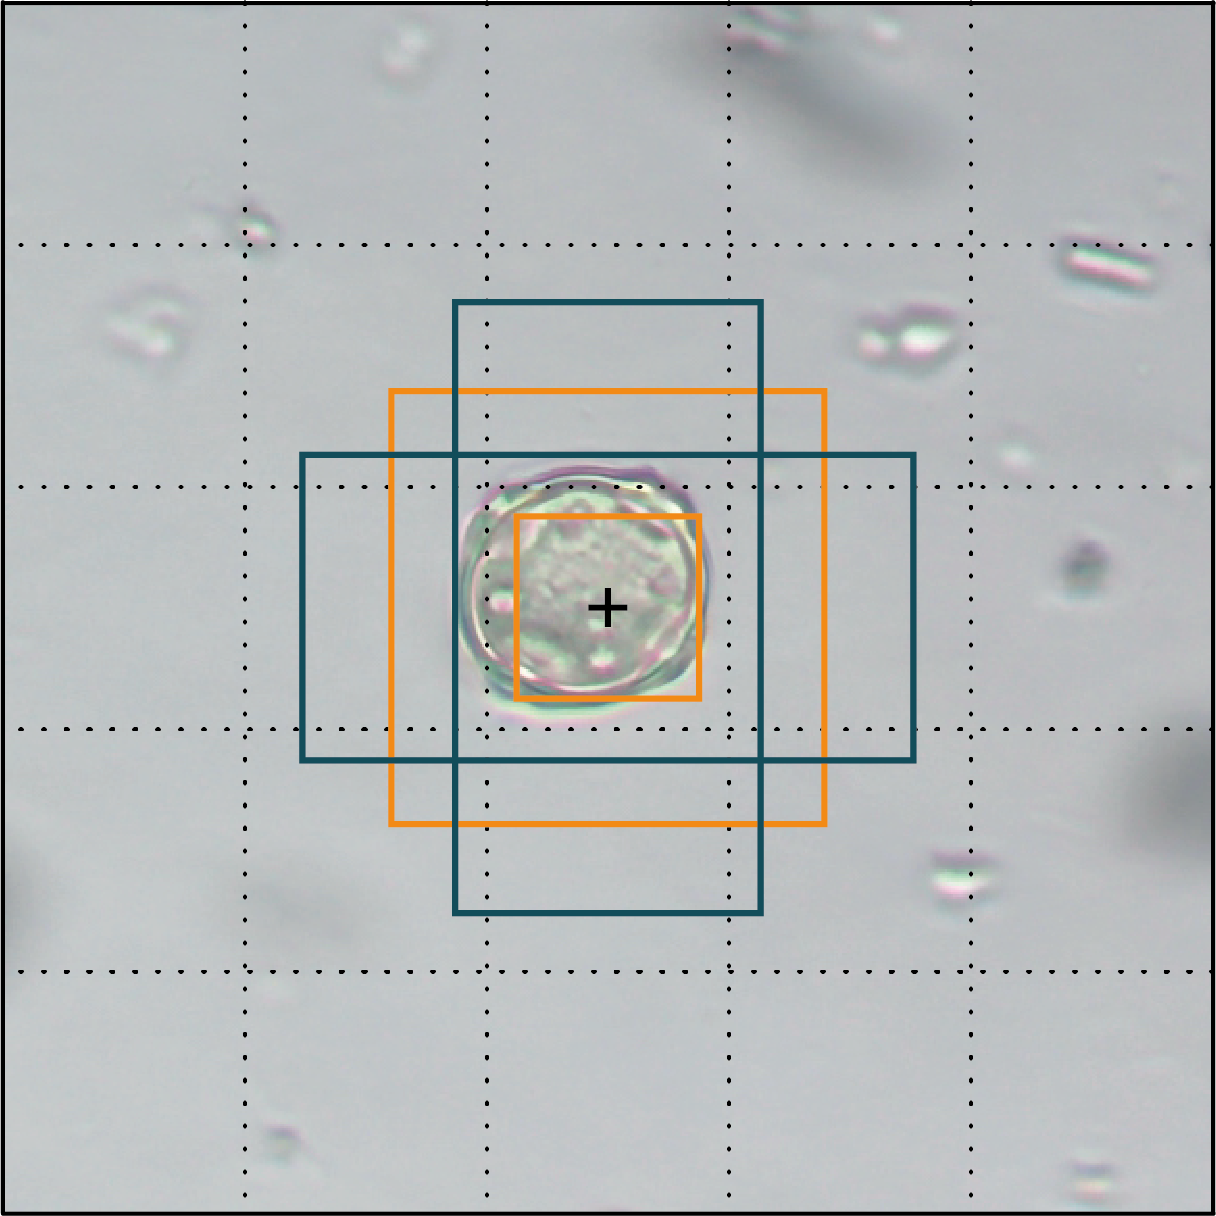
\includegraphics[width=0.4\textwidth]{figs/method/default_boxes.png}
  \caption[Visualizing default boxes]{Visualization of default boxes on a \(5\by 5 \) feature map.}\label{fig:defaults}
\end{wrapfigure}

As designed, the SSD model is made to handle a wider distribution of sizes than is present in the pollen dataset.
The sizes of the default boxes have been adjusted so that they cover the distribution of sizes present.
Even with adjustments, the range of default box sizes is so large that it is questionable if all 6 feature maps are necessary.

\subsection{Training objective}
Because of the default boxes, each ground truth box needs to be matched to one or more default boxes so that target values for the regression and confidences can be created for the loss function.
For each training example, a matching strategy is applied which finds default boxes that overlap with each ground truth.
Calculating the regression from the matched default boxes to their respective ground truth creates the truth vector that the model must approximate.

SSD has a generous matching strategy where ground truths and default boxes are matched if their IoU is above a certain threshold.
Figure~\ref{fig:priors} shows the result of the matching strategy being applied to a training example.
Every red box in the image is a default box that has been matched with a ground truth, shown in green.
For the purposes of training, these are the default boxes that the loss function expects the model to have correctly labeled and regressed.
This ensures that there are multiple positive examples for each ground truth.

\begin{figure}[htbp]
  \centering
  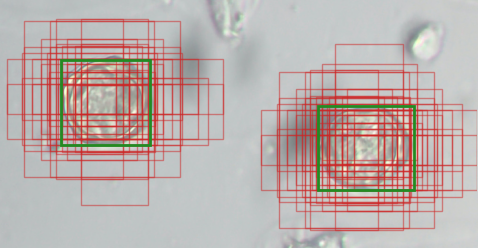
\includegraphics[width=0.7\textwidth]{figs/method/priors_matching.png}
  \caption[Default box matching]{Visualization of the result of the matching procedure.
In \textcolor{red}{red} are all the default boxes that are matched to the ground truths, i.e\ those that have an IoU \( \geq 0.4 \) with a ground truth box, in \textcolor{nicegreen}{green}.}\label{fig:priors}
\end{figure}
\info{explain lpha level\newline Not pink, only overlapping}
The loss function is calculated as follows,

\begin{equation}\label{eq:loss}
  L(x,c,l,g)=\frac{1}{N}\left( L_{conf}(x,c) + \alpha L_{loc}(x,l,g)\right)
\end{equation}

where \( x=\{1,0\} \) is a binary mask denoting a match between a default box and ground truth, \( N \) is the number of positive examples, \( c \) is class confidences, \( l \) is predicted boxes, and \( g \) is the regressed ground truth boxes.
\info{add explenation of \(g\) and regression}
\( L_{loc} \) is the summed Smooth L1 loss over all positive matched bounding boxes, while \( L_{conf} \) is the SoftMax loss over multiple class confidences, both are standard loss functions provided by PyTorch.

A problem that this and many similar models face is the gross imbalance between positive and negative training examples.
Out of the 8732 default boxes only a small subset can be matched to a ground truth.
For the localization loss this has no impact as only the matched boxes are counted towards the loss, but for the confidence the overwhelming majority of predictions are negative matches.
To counteract this imbalance SSD uses \textit{hard negative mining} to balance out the negative and positive examples.
As the name suggests, this technique aims to focus training of particularly `hard' examples and ignore the others.
All negative training examples are sorted by the confidence loss which ranks them in the order of how badly the model miss-classified them.
Negative examples are counted towards the confidence loss by descending loss until the ratio between the number of positive and negative examples included in the total loss is 1:3.

\subsection{Inference}

When the model is working, the raw output it produces is regression values for many thousands of bounding boxes with class confidence predictions.
In the locations where an object is present, the model will most likely produce multiple overlapping bounding boxes.
Ideally, the output would be a one-to-one mapping between the predicted boxes and objects in the image.

A common filtering technique is called \textit{Non-maximum Suppression} (NMS).
Let \( \mathcal{B} \) be a list of bounding boxes and \( \mathcal{S} \) be their corresponding scores.
NMS is then a simple iterative filtering algorithm where, for each iteration, the bounding box with the highest score is selected from \(\mathcal{B}\).
Any bounding boxes that overlap with the selected box are then pruned from \(\mathcal{B}\) and \(\mathcal{S}\) and the loop is continued until \(\mathcal{B}\) is exhausted.
Boxes are considered overlapping if their IoU is larger than some threshold \(N_t\).

NMS performs well in most settings, but has a particular weakness in cases where the target boxes of objects overlap.
In these situations, NMS will often only return a single bounding box for one of the objects, ignoring the rest.
Given that the data in this project exhibits this characteristic, the standard NMS algorithm is replaced with a more modern version, Soft-NMS, introduced in\ \textcite{bodla2017softnms}.
The pseudocode for both algorithms is as follows,

\begin{pseudofunc}{NMS}{\(\mathcal{B}=\{b_1,\ldots,b_N \},~\mathcal{S}=\{s_1,\ldots,s_N \},~N_t\)}
  \item \(\mathcal{D} \leftarrow \{ \} \)
  \item \pwhile~\(\mathcal{B} \neq \emptyset \):
  \begin{pseudoloop}
    \item \(m \leftarrow \text{argmax}~\mathcal{S}\)
    \item \(\mathcal{M} \leftarrow b_m\)
    \item \(\mathcal{D} \leftarrow \mathcal{D} \cup \mathcal{M};~ \mathcal{B} \leftarrow \mathcal{B} - \mathcal{M}\)
    \item \pfor~\(b_i \in \mathcal{B}\):
    \vspace{6pt}
    \begin{pseudoloop}
      \fcolorbox{red}{white}{\color{red} %
      \minipage[t]{\dimexpr0.50\linewidth-2\fboxsep-\fboxrule\relax}
        \item \pif~\pmethod{IoU}{\(\mathcal{M},~b_i\)}\(~\geq N_t\):
        \item \(~~\mathcal{B} \leftarrow \mathcal{B} - b_i;~ \mathcal{S} \leftarrow \mathcal{S} - s_i\)
        \vspace{3pt}
        \begin{textblock}{1} (3.7,-0.15)
          \textcolor{black}{\texttt{NMS}}
        \end{textblock}
      \endminipage}\vspace{5pt}\\
      \fcolorbox{nicegreen}{white}{\color{nicegreen}%
      \minipage[t]{\dimexpr0.50\linewidth-2\fboxsep-\fboxrule\relax}
        \item \(s_i \leftarrow s_i\)\pmethod{f}{\pmethod{IoU}{\(\mathcal{M},~b_i\)}}
        \begin{textblock}{2} (3,-0.15)
          \textcolor{black}{\texttt{Soft-NMS}}
        \end{textblock}
      \endminipage}
    \end{pseudoloop}
  \end{pseudoloop}\vspace{5pt}
  \item \pret~\(\mathcal{D},~\mathcal{S}\)
\end{pseudofunc}

\begin{wrapfigure}[13]{r}{0.3\textwidth}
  \centering
  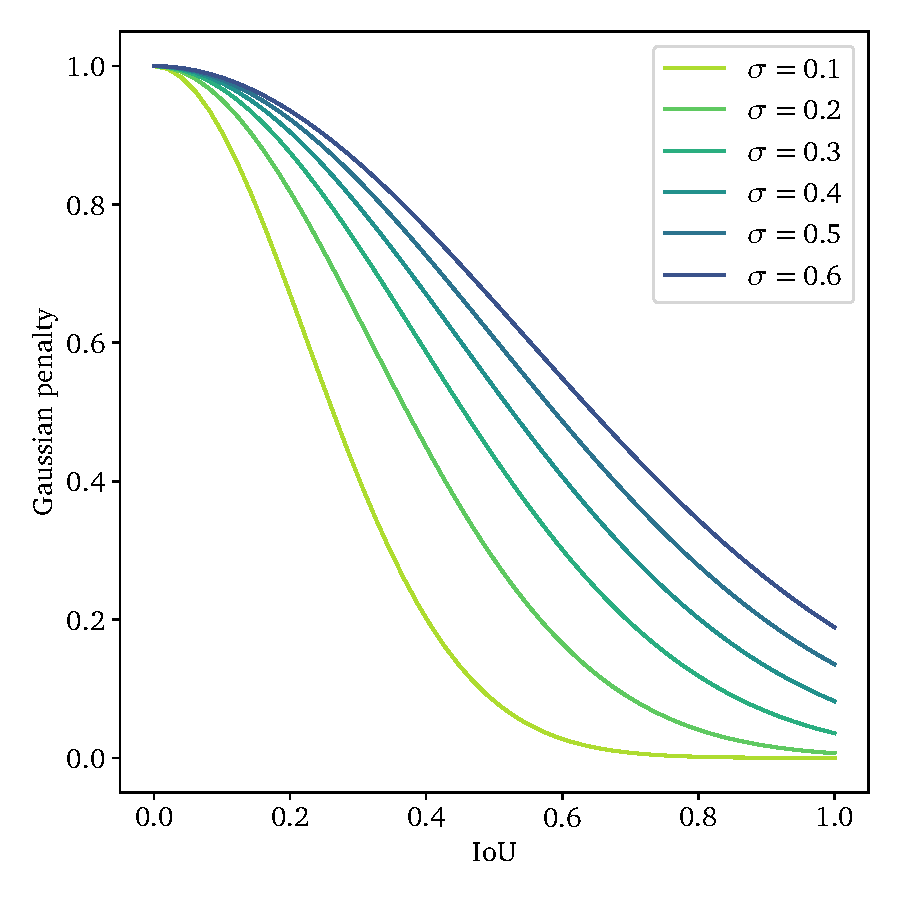
\includegraphics[width=0.3\textwidth]{figs/method/gausian_penelty.pdf}
  \caption{Gaussian decay as a function of IoU for various \( \sigma \)}\label{fig:gauss}
\end{wrapfigure}

Soft-NMS changes only the colored sections, where it introduces a rescoring function, \texttt{f(IoU)}, which only decays the scores of remaining boxes instead of discarding them altogether. % chktex 36
This allows boxes which overlap with the selected box to remain in the pool.
Rescoring is applied using a Gaussian decay function as follows,

\[s_i\leftarrow s_i e^{-\frac{\text{iou}{(\mathcal{M}, b_i)}^2}{\sigma}},~~\forall b_i \notin \mathcal{D}\]

where \( \sigma \) controls the rate of decay, as demonstrated in Figure~\ref{fig:gauss}.
\info{define all terms}

\section{Experimental setup}\label{sec:method-exp-setup}
This section will present the experiments which have been designed in order to examine the research questions.
Firstly, the software and hardware stack used in the implementation of the model is presented, as well as the training procedure used for the experiments.
A run-down of the experiments that have been performed will then be given.

\subsection{Software}
All of the software for this project has been written in Python which is among the most established languages for the purposes of deep learning.
This project relies entirely on the extensive use of the high quality open source data science ecosystem that has been created within Python.
The model implementation, training, and evaluation procedures are written using the 1.7 release of the PyTorch library\ \parencite{NEURIPS2019_9015}.
PyTorch is an extensive machine learning framework and provides APIs covering the entire model pipeline.

\subsection{Hardware}
All experiments have been run on a desktop computer using consumer grade components.
The relevant specifications are as follows,
\begin{itemize}
  \item \textbf{CPU:} \textit{AMD Ryzen 5 3600X}, 6 cores @ 3.8 GHz.
  \item \textbf{GPU:} \textit{Nvidia GTX 1070}, 8 GB GDDR5 VRAM,\\1920 CUDA cores @ 1506 MHz, 6.463 TFLOPS (32 bit).
  \item \textbf{Memory:} \textit{Corsair Vengeance}, 32 GB DDR4 @ 2166 MHz.
\end{itemize}
{\it
\textcolor{red}{Summary of training time and model speed re inference}
}
\subsection{Training}
All the experiments where run using the same training setup.
The model is trained using Stochastic Gradient Decent (SGD) with a mini batch size of 32, learning rate of \num{e-3}, \num{0.9} momentum, and \num{5e-4} weight decay.
In testing, test mAP converged after 2000 iterations in the baseline configuration

The dataset contains tree classes, but these are not equally distributed between the 701 images.
Corylus and Alnus both release together and are found together in samples.
Poaceae appears as the only class in the samples where it is present, it is also much more prevalent than the other species meaning the density of pollen grains is much higher on average in these samples.
This also causes the very uneven distribution of classes in the dataset.
The Poaceae class is therefore under-sampled when creating the final dataset.
467 samples are included in the final dataset, the class distribution is given in Table~\ref{tab:training-dataset}.
The final dataset is then divided into a training and test split with a 85\% / 15\% ratio.

\begin{table}[htbp]
  \caption[Class distribution across the final training dataset containing 467 sample images.]{Distribution of classes across the training dataset}\label{tab:training-dataset}
  \centering
  \begin{tabular}{lrrr} \toprule
                      & Poaceae & Corylus & Alnus \\ \midrule
    Number of labels  & 518    & 262     & 522 \\
    Share             & .40  & .20  & .40 \\ \bottomrule
  \end{tabular}
\end{table}

Augmentations are necessary to allow the model to train for many enough iterations without overfitting on the training set.
Augmentations artificially increase the size of the dataset, by producing thousands of variations of each example.
The following augmentations are employed,
%
\begin{enumerate}
  \item Horizontal flip.
  \item Vertical flip.
  \item Color adjustment (brightness, hue, saturation, contrast).
  \item Shuffle RBG channels.
  \item Random crop.
\end{enumerate}
%
All the augmentations except cropping, independently, have a 50\% chance of being applied to each sample.
Random crop also resizes the sample input into a \(300\by 300\) square so it is needed for every image.
The cropping algorithm also ensures that each sample contains at least one pollen grain.

\section{Experiments}\label{sec:method-experiments}
Four experiments are designed, two targeting each research question.
With the goal of developing a system for automated pollen counting, the aim is to explore how the peculiarities of this domain interact with the more established methods that have been developed for object detection.
For each experiment its rational and setup is given.

\subsection{Feature extractor}
The largest section of the model is the feature extraction block, so with the goal of decreasing computational complexity, shrinking this block would have the largest impact.
Because this dataset differs so much from the common datasets used to pre-train the feature extractors, it is difficult to predict the impact from using a smaller network.
On one hand the dataset is more uniform with similar backgrounds for every image, on the other hand all pollen grains look similar to each other so depth might be necessary to differentiate between them.
In the first experiment the model is trained with three different pre-trained feature extraction networks and compare them.
The selected networks are given in Table~\ref{tab:ex01}

\begin{table}[htbp]\centering
  \ra{1.2}
\caption[Feature extraction networks]{Chosen feature extraction networks and relative size calculated by number of trainable parameters}%
\label{tab:ex01}
\begin{tabular}{@{}lr@{}}\toprule
  Network & Relative size \\
  \midrule
     ResNet 34 & 1.00  \\
     ResNet 18 & 0.34  \\
  MobileNet V2 & 0.02  \\
  \bottomrule
\end{tabular}
\end{table}

\subsection{Layer activation}
The auxiliary structure also has opportunities for simplification.
The main rational for SSD's multiple stacked feature maps is to allow for predictions at multiple scales in the image.
Pollen grains however appear very uniform in size and shape throughout the dataset.
The hypothesis is that some or most of the source feature maps can be removed from the model without any performance degradation.
To test this the model will be trained in multiple configurations where certain feature maps from the model are removed for each configuration.
In practice, only the detection blocks that are fed by the feature maps are deactivated, so that layers can be arbitrarily deactivated without disturbing successive layers of the model.

\subsection{Minimum training sharpness}
As observed, the dataset contains a wide variety of grains spanning many levels of blur.
It remains unclear what impact blurry data has on the training of fully convolutional object detection systems.
With this experiment the aim is to explore if there is a correlation between the distribution of sharpness in the training data and model predictions.
The performance of the model is not of interest, but rather how the distribution of sharpness values in the training data changes the distribution of sharpness in the predictions.
Sharpness can be measured both on the predictions of the model and on the ground truths it does or does not detect.
\done{Confusing. Split sentence in two}

For the experiment the model is trained on various versions of the same dataset.
Each model will be trained on a subset of the ground truth labels using a sharpness filter which prunes any ground truth bellow a certain threshold.
Raising the threshold limits the model to only those pollen grains sharper than the threshold.
5 thresholds are used, spanning a range from 0 to 0.08 which covers the lower half of sharpness values contained in the dataset.

\subsection{Cross-sharpness inference}
The final experiment aims to further explore what ability the model has to generalize outside of the sharpness values it is exposed to, and whether or not a trained model can be transferred to different sharpness ranges.
Similar to the previous experiment the model is trained on a subset of ground truths, one with only the sharp ground truths and one with only the blurry ground truths.
The same partition is also applied to the testing split.
Together with a baseline containing all ground truths, three models and three test splits are created.
Each of the three models will be tested on each of the three test partitions, creating a kind of sharpness confusion matrix.
